% ===== UNIT 24: Seed variance + fusion-weight sensitivity (5.5-5.6) =====
% Status: REWRITTEN  (change to REWRITTEN / REVIEWED when done; see CHECKLIST.md)
% Rules: style rewrite only. Keep every \cite, \ref, \label, number, equation and table value as is. Change the wording, not the content.
\subsection{Training seed variance}
\label{sec:seed_variance}
To measure training-time randomness, we retrained the A5$\alpha$ recipe from scratch with three additional seeds $\{42, 123, 456\}$ under identical hyperparameters. Each run was evaluated at the isolated-ablation operating point (Stream~1 only, single-flip 768D, AQE $k{=}3$ $+$ $k$-reciprocal re-ranking, Table~\ref{tab:ablation}, top block). Table~\ref{tab:seed_variance} bounds the training variance of the recipe. This supports the argument that A5$\alpha$ and A5$\beta$ are equivalent. It is not a re-derivation of the released headline checkpoint, whose reproducibility is established separately (below).

\begin{table}[!t]
  \centering
  \caption{A5$\alpha$ training seed variance on VeRi-776 (Stream~1 only,
    single-flip 768D, AQE $k{=}3$ $+$ $k$-reciprocal re-ranking), quantifying
    from-scratch retraining noise of the recipe}
  \label{tab:seed_variance}
  \small
  \begin{tabular}{L{4.6cm}C{3.0cm}C{3.0cm}}
    \toprule
    Seed & mAP~(\%) & R1~(\%) \\
    \midrule
    42  & 89.48 & 97.26 \\
    123 & 88.14 & 97.08 \\
    456 & 88.64 & 97.20 \\
    \midrule
    \textbf{Mean $\pm$ SD ($n=3$)} & \textbf{88.75 $\pm$ 0.55} & \textbf{97.18 $\pm$ 0.07} \\
    \bottomrule
  \end{tabular}
\end{table}

The three-seed standard deviation of 0.55\,pp mAP is larger than the 0.49\,pp single-run gap between A5$\alpha$ and A5$\beta$. So the two recipes are statistically equivalent under realistic training noise. This is purely a training-time analysis. The headline Stream~1 result (89.97\% mAP) is not the mean of these retrains. It is the deterministic evaluation of the released, SHA-pinned checkpoint at the best-mAP operating point (1536D concat-patch flip TTA). Its reproducibility is therefore exact. The same frozen checkpoint gives the same number on every run, regardless of training variance. This is the guarantee we provide by releasing the checkpoint. For transparency, that checkpoint scores 89.63\% at the 768D operating point of this table, which is at the favourable end of the retrain distribution. A reproducer who trains from scratch should expect the band above. A reproducer who evaluates the released checkpoint gets the headline exactly.

\subsection{Fusion weight sensitivity}
\label{sec:weight}
Figure~\ref{fig:weight} sweeps the fusion weight. The mAP stays above 93.0\% for $w_1 \in [0.2, 0.5]$, so the result does not depend much on the exact weight. Every fusion configuration is better than either stream alone. This confirms that the two streams capture complementary information about vehicle identity.

\begin{figure}[!t]
  \centering
  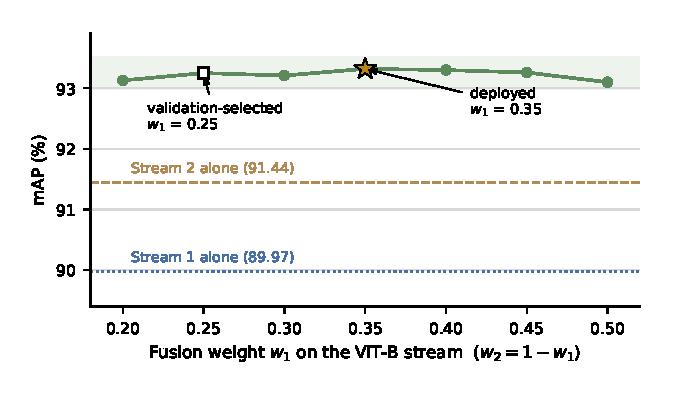
\includegraphics[width=0.92\columnwidth]{Fig7}
  \caption{Fusion weight sensitivity on VeRi-776. The fused mAP stays within
  0.22\,pp across the entire range $w_1 \in [0.2, 0.5]$ and everywhere exceeds
  both single streams, so the reported result does not sit on a sharp test-set
  optimum. The star marks the deployed weight and the open square the weight
  selected on a disjoint identity split (Section~\ref{sec:holdout})}
  \label{fig:weight}
\end{figure}

We also checked that the Stream~1 feature dimensionality has almost no effect on the fused result. The 1536D concat-patch flip-TTA representation and the 768D single-flip CLS-only representation fuse to within 0.01\,pp mAP at their respective optima (1536D: 93.32\% at $w_1{=}0.35$, 768D: 93.31\% at $w_1{=}0.30$). This is true even though the 1536D representation is 0.34\,pp stronger on its own (89.97\% vs.\ 89.63\%). So the standalone TTA gain is largely redundant with the complementary CLIP-SENet signal. We keep the 1536D representation, because it is the best-mAP standalone Stream~1 configuration and is also slightly best in fusion.
